\documentclass[sans,mathserif,aspectratio=169]{beamer}

\usepackage{booktabs}
\usepackage[spanish, mexico]{babel}
\selectlanguage{spanish}
\decimalpoint
\usepackage[utf8]{inputenc}
\usepackage{tikz}
\usepackage{fourier}
\newcommand{\quotes}[1]{``#1''}
\usepackage{epstopdf}
\usepackage{mathtools}
\DeclarePairedDelimiter{\ceil}{\lceil}{\rceil}
\usepackage{commath}
\usepackage{amsmath,tabularx}
\usepackage{listings}
\usepackage{xcolor}
\usepackage[edges]{forest}
\graphicspath{{Images/}}
\usepackage[mathscr]{euscript}

\definecolor{foldercolor}{RGB}{124,166,198}

\tikzset{pics/folder/.style={code={%
    \node[inner sep=0pt, minimum size=#1](-foldericon){};
    \node[folder style, inner sep=0pt, minimum width=0.3*#1, minimum height=0.6*#1, above right, xshift=0.05*#1] at (-foldericon.west){};
    \node[folder style, inner sep=0pt, minimum size=#1] at (-foldericon.center){};}
    },
    pics/folder/.default={20pt},
    folder style/.style={draw=foldercolor!80!black,top color=foldercolor!40,bottom color=foldercolor}
}

\forestset{is file/.style={edge path'/.expanded={%
        ([xshift=\forestregister{folder indent}]!u.parent anchor) |- (.child anchor)},
        inner sep=1pt},
    this folder size/.style={edge path'/.expanded={%
        ([xshift=\forestregister{folder indent}]!u.parent anchor) |- (.child anchor) pic[solid]{folder=#1}}, inner xsep=0.6*#1},
    folder tree indent/.style={before computing xy={l=#1}},
    folder icons/.style={folder, this folder size=#1, folder tree indent=3*#1},
    folder icons/.default={12pt},
}

\colorlet{punct}{red!60!black}
\definecolor{background}{HTML}{EEEEEE}
\definecolor{delim}{RGB}{20,105,176}
\colorlet{numb}{magenta!60!black}

\lstdefinelanguage{json}{
    basicstyle=\normalfont\ttfamily\tiny,
    columns=flexible,
    keepspaces=true,
    frame=lines,
    backgroundcolor=\color{background}
}

\mode<presentation>

%Colors
\definecolor{steel}{RGB}{52,102,136}
\definecolor{moss}{RGB}{139,187,159}
\definecolor{burnt}{RGB}{187,102,65}
\definecolor{sandy}{RGB}{186, 168, 111}
\definecolor{RoyalBlue}{RGB}{0,35,102}
\definecolor{cream}{RGB}{254, 246, 235}
\definecolor{slate}{RGB}{82, 85, 100}
\definecolor{fall}{RGB}{194, 91, 86} % frame color
\definecolor{light}{RGB}{150, 192, 206}

%Structure
\usefonttheme{professionalfonts}
\hypersetup{colorlinks,linkcolor=fall!80,urlcolor=fall!80}
\setbeamercolor{local structure}{fg=fall}
\setbeamercolor{background canvas}{bg=cream}
\setbeamercolor{frametitle}{bg=fall,fg=cream}
\setbeamercolor{title}{fg=steel!115}
\setbeamercolor{author}{fg=fall}

\defbeamertemplate*{title page}{customized}[1][]
{\centering
  %\frame{
\includegraphics[width=0.80\linewidth]{article_cover.jpeg}}
  \fcolorbox{fall}{white}{
\includegraphics[width=0.80\linewidth]{article_cover.jpeg}}
  \vfill
  \usebeamerfont{author}\usebeamercolor[fg]{author}\insertauthor\par
  \vfill
  \usebeamerfont{institute}\insertinstitute\par
  \usebeamerfont{date}\insertdate\par
  \usebeamercolor[fg]{titlegraphic}\inserttitlegraphic
}

% Progressbar
\usepackage{tikz}
\usetikzlibrary{calc}

\makeatletter
\def\progressbar@progressbar{} % the progress bar
\newcount\progressbar@tmpcounta% auxiliary counter
\newcount\progressbar@tmpcountb% auxiliary counter
\newdimen\progressbar@pbht %progressbar height
\newdimen\progressbar@pbwd %progressbar width
\newdimen\progressbar@tmpdim % auxiliary dimension

\progressbar@pbwd=\paperwidth
\progressbar@pbht=2pt

\def\progressbar@progressbar{%

\progressbar@tmpcounta=\insertframenumber
\progressbar@tmpcountb=\inserttotalframenumber
\progressbar@tmpdim=\progressbar@pbwd
\multiply\progressbar@tmpdim by \progressbar@tmpcounta
\divide\progressbar@tmpdim by \progressbar@tmpcountb

  \begin{tikzpicture}[very thin]

  \shade[draw=steel!115,top color=steel,bottom color=steel,middle color=steel!115] %
    (0pt, 0pt) rectangle ++ (\progressbar@tmpdim, \progressbar@pbht);

  \end{tikzpicture}%
 }

\addtobeamertemplate{frametitle}{}
{%
  \vspace*{-16pt}
  \begin{beamercolorbox}[wd=\paperwidth,ht=1pt,dp=1pt]{}%
    \progressbar@progressbar%
  \end{beamercolorbox}%
}%
\makeatother

%Title
\title{Code Development Environment}
\subtitle{Experiences and Outlook}
\author[Guillermo Ibarra]{Guillermo Ibarra}
\date{Nuclear Engineering Research Seminar, February 25th, 2020}

\definecolor{keywords}{RGB}{255,0,90}
\definecolor{comments}{RGB}{0,0,113}
\definecolor{red}{RGB}{160,0,0}
\definecolor{green}{RGB}{0,150,0}

\setbeamercovered{transparent}
\setbeamercovered{%
  again covered={\opaqueness<1->{40}}}
\beamertemplatenavigationsymbolsempty


\begin{document}

%slide
\begin{frame}
\titlepage
\end{frame}

%slide
\begin{frame}{Introduction}
\begin{equation*}
\hat{\Omega}_m \cdot \nabla \psi_{g,m} \left(  \vec{r} \right) + \Sigma_{t,g}\psi_{g,m} \left( \vec{r} \right) = \frac{1}{4\pi} \left[\sum\limits_{g'=1}^{G} \Sigma_{s, g' \to g} \phi_{g'} \left( \vec{r} \right) + \frac{\chi_g}{k_{e\!\!f\!\!\!f}} \nu \Sigma_{f, g'} \phi_{g'}  \left( \vec{r} \right) \right],
\end{equation*}
\pause
where
\begin{equation*}
\phi_g = \sum_m \psi_{g,m} w_m.
\end{equation*}
\end{frame}

%slide
\begin{frame}{Operator Notation}
\begin{equation*}
\mathscr{L} \Psi = \frac{1}{4\pi} \left[ \mathscr{S} + \frac{1}{k_{e\!\!f\!\!\!f}} \mathscr{F} \right] \Phi,
\end{equation*}
where:
\begin{align*}
\mathscr{L} &= \hat{\Omega} \cdot \nabla + \Sigma_t \\
\mathscr{S} &= \Sigma_s  \\
\mathscr{F} &= \chi \nu \Sigma_f
\end{align*}
and
\begin{align}
\Psi &= \left[ \psi_1, \psi_2, \dotso, \psi_G \right] \nonumber \\
\Phi &= \left[ \phi_1, \phi_2, \dotso, \phi_G \right] \nonumber \\
\phi &= \mathscr{M}_0 \psi \nonumber
\end{align}
\end{frame}

%slide
\begin{frame}{Power Iteration}
\centering
\fcolorbox{fall}{white}{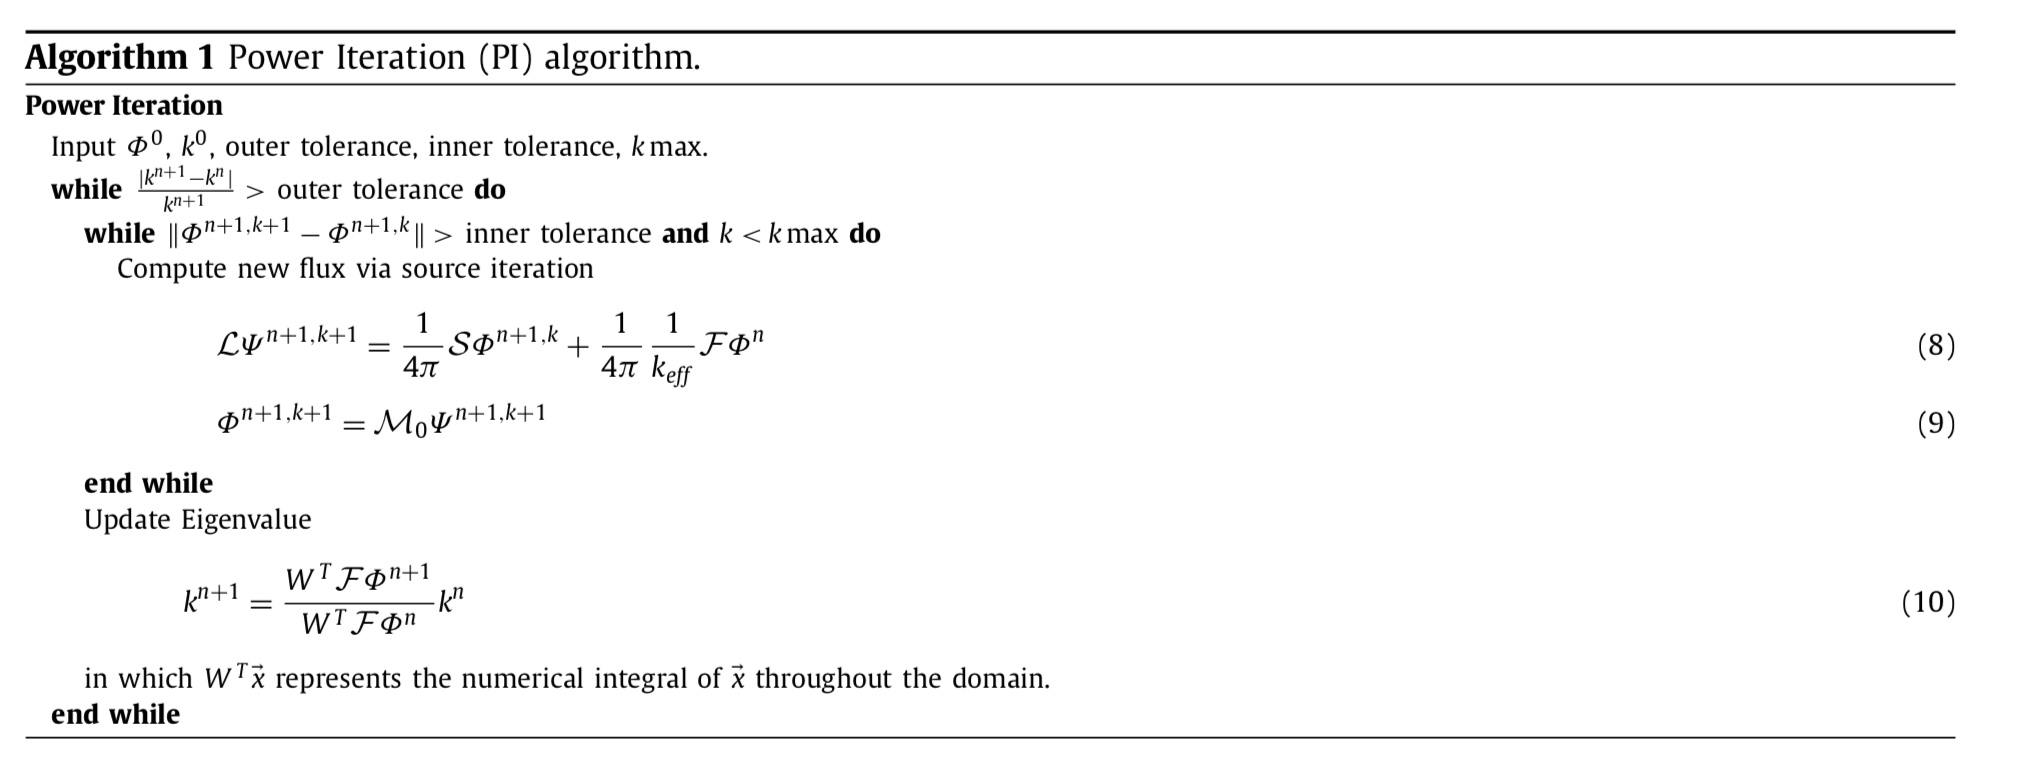
\includegraphics[width=0.95\linewidth]{algo1.jpeg}}
\end{frame}

%slide
\begin{frame}{Housekeeping}
\begin{itemize}
  \item<1> JFNK: Jacobian-Free Newton-Krylov
  \item<1> NKA: Nonlinear Krylov Acceleration
  \item<2> HOLO: High-Order/Low-Order Acceleration, Moment Base Acceleration
  \item<2> NDA: Nonlinear Diffusion Acceleration
\end{itemize}
\end{frame}

%slide
\begin{frame}{Motivation}
H. Park, D.A, Knoll, C.K. Newman,\emph{Nonlinear acceleration of transport criticality problems}, 
Nucl. Sci. Eng. 172 (2012) 53-56
\begin{itemize}
  \item NDA to accelerate scattering source
  \item JFNK to accelerate the fission source in LO space
\end{itemize}
\end{frame}

%slide
\begin{frame}{First Test}{$\tau = 15$}
\centering
\fcolorbox{fall}{white}{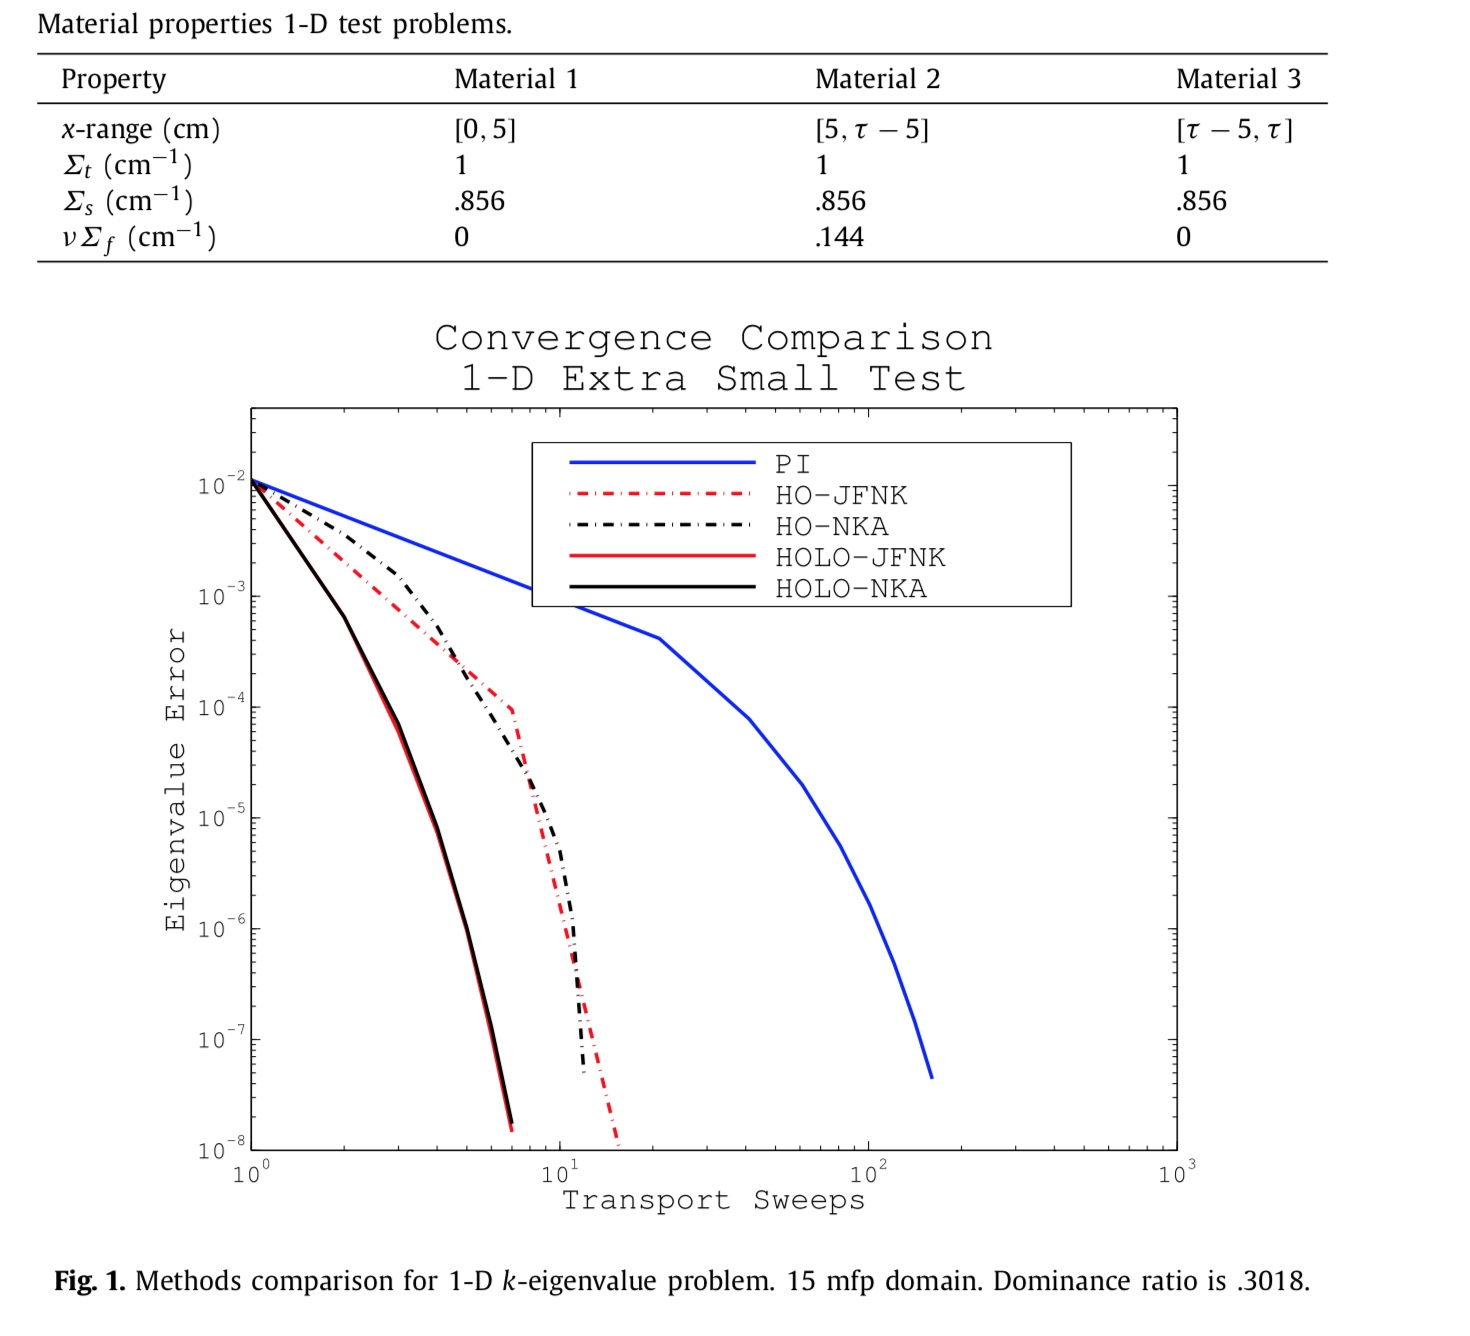
\includegraphics[width=0.55\linewidth]{motivation.jpeg}}
\end{frame}

%slide
\begin{frame}{First Test}{$\tau = 35$ and $\tau = 210$}
\begin{minipage}{0.45\textwidth} 
    \centering
    \fcolorbox{fall}{white}{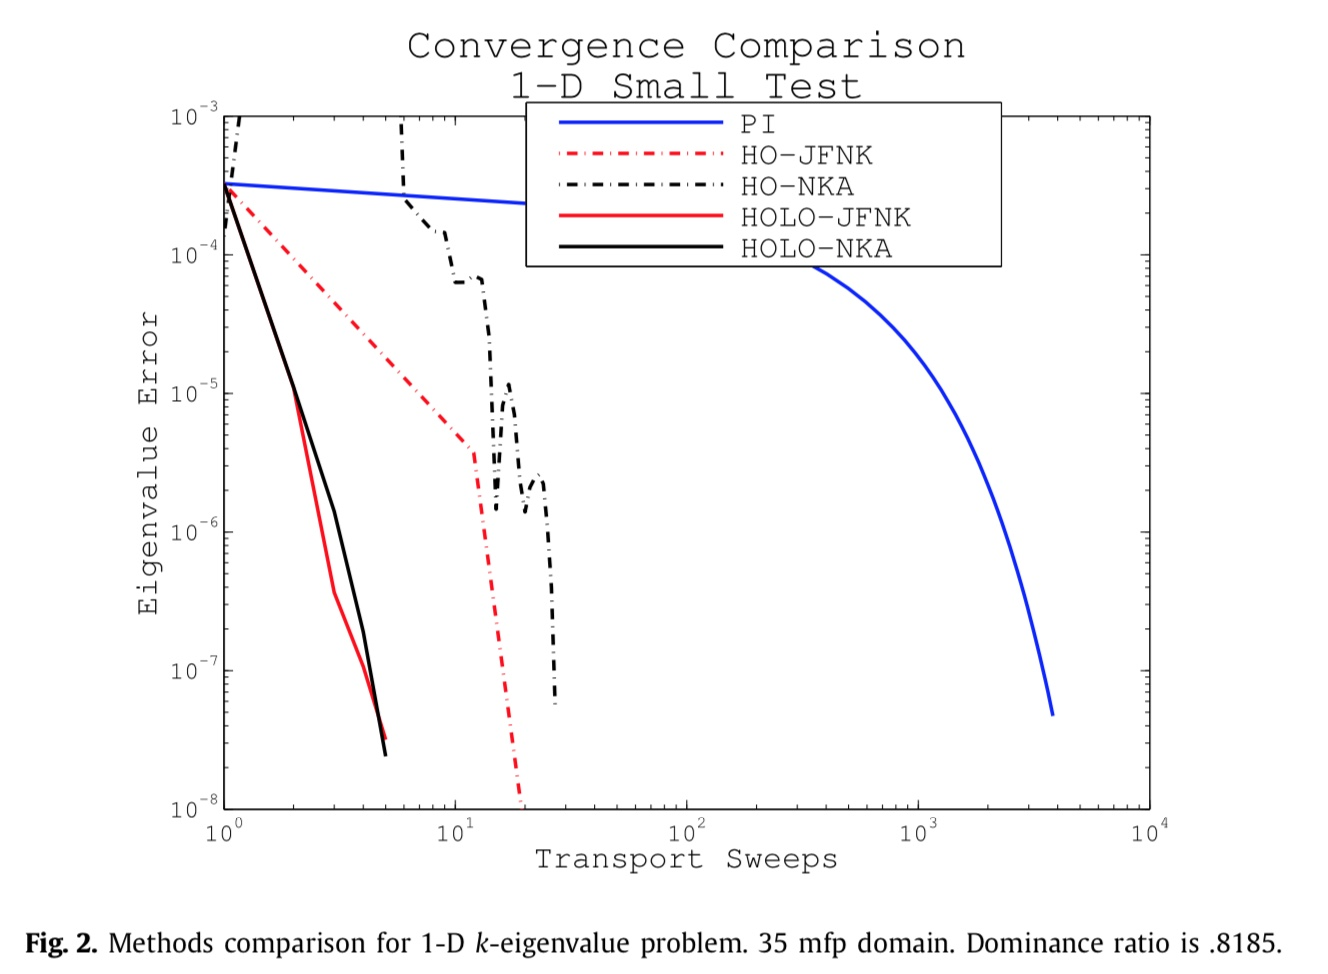
\includegraphics[width=\linewidth]{fig2.jpeg}}
\end{minipage}
\qquad
\pause
\begin{minipage}{0.45\textwidth}
    \centering
    \fcolorbox{fall}{white}{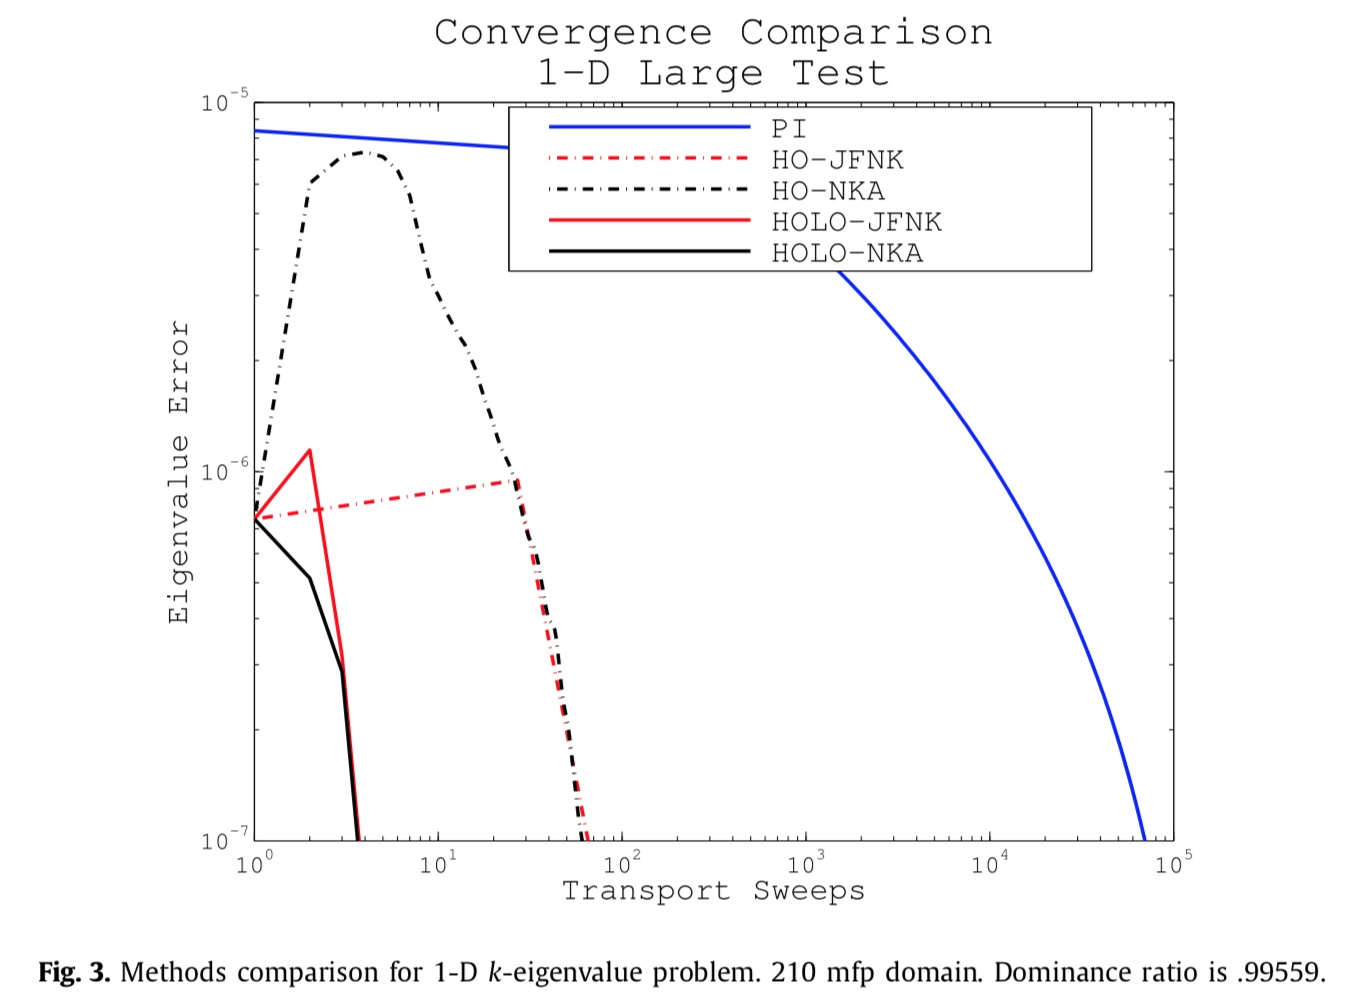
\includegraphics[width=\linewidth]{fig3.jpeg}}
\end{minipage}
\end{frame}

%slide
\begin{frame}{Nonlinear Acceleration of Transport Criticality Problems}
\begin{equation}
   F
   \begin{pmatrix}
     \Phi \\
      k
   \end{pmatrix}
   =
   \begin{pmatrix}
     F_\Phi (\Phi, k) \\
     F_k (\Phi, k)
   \end{pmatrix}
   =
   0
\end{equation}
\end{frame}

%slide
\begin{frame}{Nonlinear Acceleration of Transport Criticality Problems}{function aproximations}
\begin{align*}
 \onslide<1-> {F_\Phi (\Phi, k) &= \Phi - P(k)\Phi \\}
 \onslide<2> {P_1(k) &= \mathscr{M}_0 \mathscr{L}^{-1} \left[\frac{1}{4\pi} \left( \mathscr{S} + \frac{1}{k}\mathscr{F} \right)\right] \\}
 \onslide<3> { \Phi^{n+1} &= P_2(k^n)\Phi^n \\
 P_2(k^n)\Phi^n &= \mathscr{M}_0 \left( \mathscr{L} - \frac{1}{4\pi}\mathscr{S}\mathscr{M}_0 \right)^{-1}\frac{1}{4\pi k^n} \mathscr{F}\Phi^n \\}
 \onslide<4> {F_k (\Phi, k) &= \left( 1 - \frac{W^T\mathscr{F} P(k)\Phi}{W^T\mathscr{F}\Phi} \right) k}
\end{align*}
\end{frame}

%slide
\begin{frame}{JFNK Algorithm}
\centering
\fcolorbox{fall}{white}{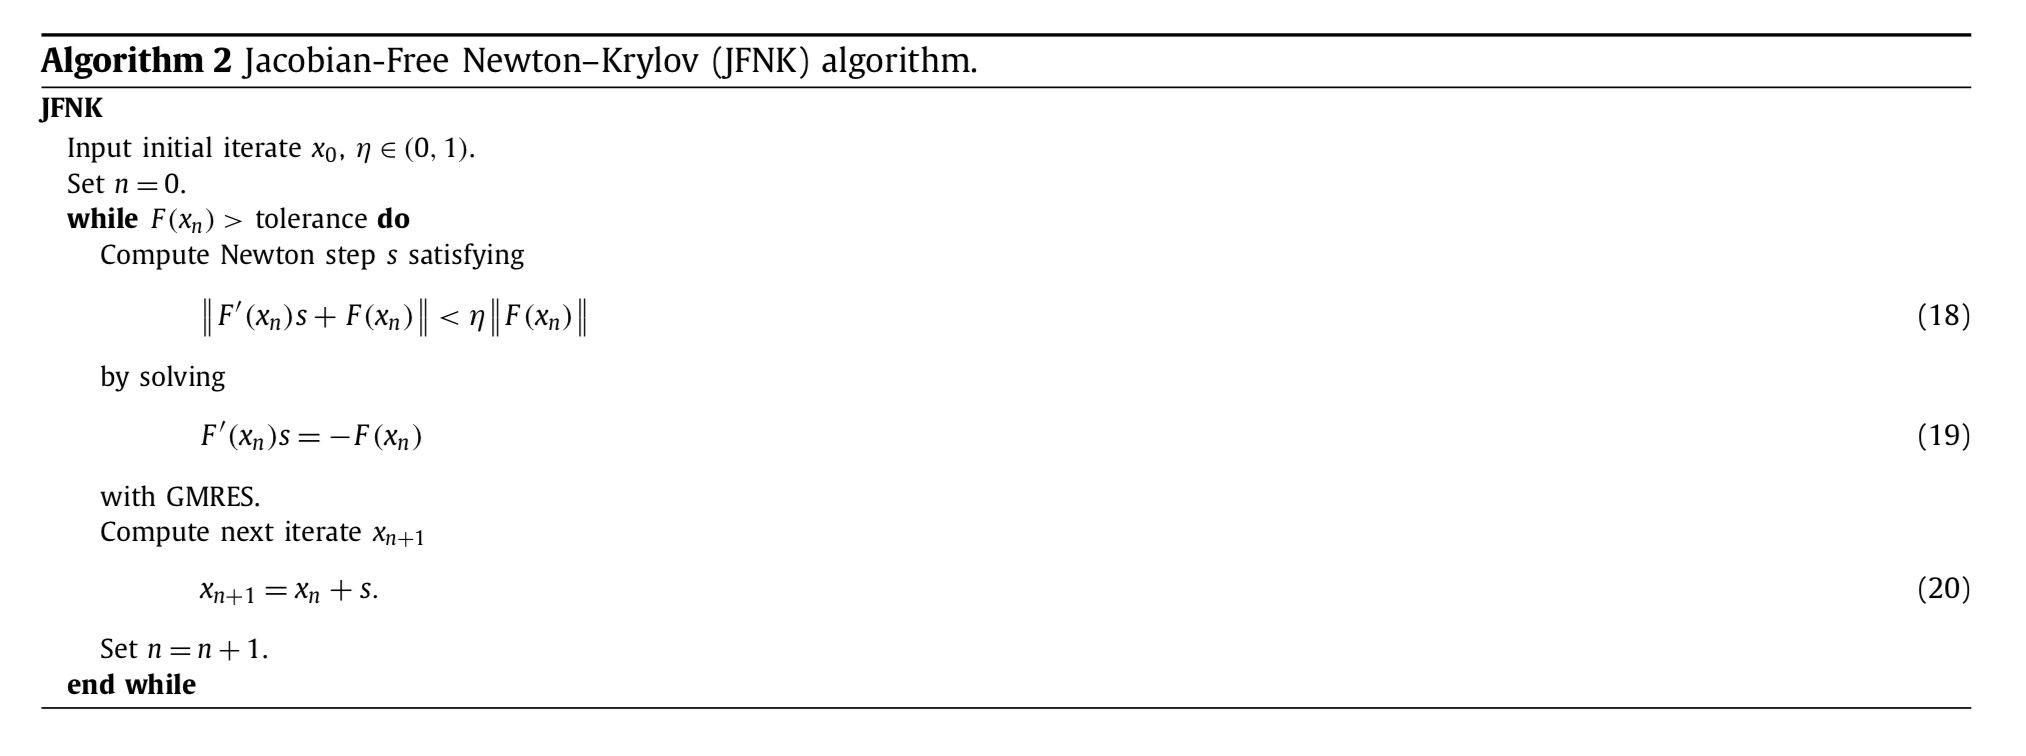
\includegraphics[width=0.95\linewidth]{algo2.jpeg}}
\end{frame}

%slide
\begin{frame}{NKA Algorithm}
\centering
\fcolorbox{fall}{white}{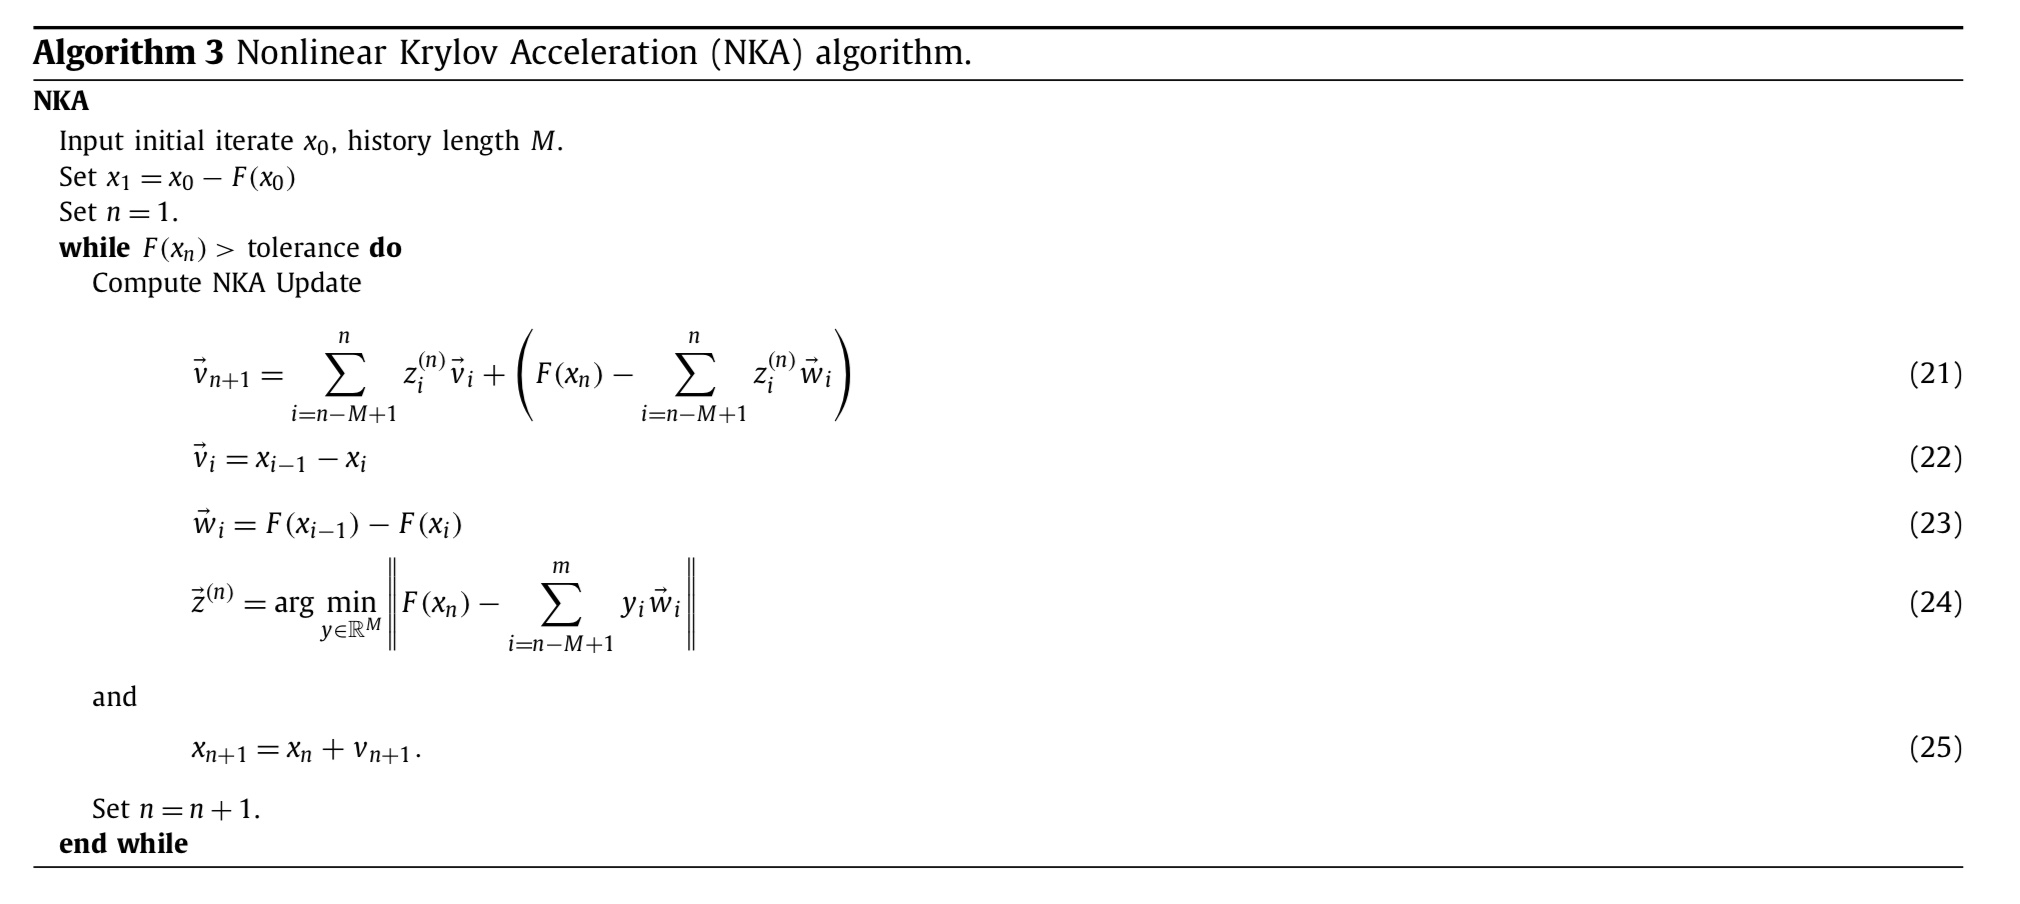
\includegraphics[width=0.95\linewidth]{algo3.jpeg}}
\end{frame}

%slide
\begin{frame}{Nonlinear Elimination of the Eigenvalue}
\begin{equation*}
Ax = \lambda x
\end{equation*}
such that $(\lambda^*, x^*)$ and $(\lambda^*, cx^*)$ are pairs; with the constraint $\left\lVert x^*\right\rVert = 1$.
\pause
\begin{align*}
\onslide<2> {k &= \int \int \nu \Sigma_f \phi dV dE \\}
\onslide<3-> {F(\Phi) &= \Phi - P\left( k \left( \Phi \right) \right) \Phi \\}
\onslide<4-> {k \left( \Phi \right) &= \int \int \nu \Sigma_f \phi dV dE}
\end{align*}
\end{frame}

%slide
\begin{frame}{HOLO Methods}
\begin{align*}
\onslide<1-> {&\nabla \cdot \vec{J}_g + \left( \Sigma_{t,g} - \Sigma_{s,g \to g} \right) \phi_g = \sum_{g'\ne g} \Sigma_{s, g' \to g} \phi_{g'} + 
              \frac{\chi_g}{k_{e\!\!f\!\!\!f}} \sum_{g'=1}^G \nu \Sigma_{f,g'} \phi_{g'} \\}
\onslide<2> {&\vec{J}_g (\vec{r}) = \int_{4\pi} \vec{\Omega} \psi_g \left( \vec{\Omega}, \vec{r} \right) d\vec{\Omega} = \mathscr{M}_1 \psi_g\\}
\onslide<3> {&\vec{J}_g = -\frac{1}{3\Sigma_{t,g}}\nabla \psi_g + \vec{D}_g \phi_g \\}
\onslide<4-> {&\nabla \cdot \left[ -\frac{1}{3\Sigma_{t,g}}\nabla \psi_g + \vec{D}_g \phi_g \right] + \left( \Sigma_{t,g} - \Sigma_{s,g \to g} \right) \phi_g 
              = \sum_{g'\ne g} \Sigma_{s, g' \to g} \phi_{g'} + \frac{\chi_g}{k_{e\!\!f\!\!\!f}} \sum_{g'=1}^G \nu \Sigma_{f,g'} \phi_{g'}}
\end{align*}
\end{frame}

%slide
\begin{frame}{HO Moments}
Consistency term:
\begin{equation*}
 \vec{D}_g = \frac{\vec{J}_g^{HO} + \frac{1}{3\Sigma_{t,g}} \nabla \phi_g^{HO}}{\phi_g^{HO}}
\end{equation*}
\pause
From the transport sweep:
\begin{align*}
\onslide<2-> {&\Psi = \frac{1}{4\pi} \mathscr{L}^{-1} \left[ \mathscr{S} + \frac{1}{k_{e\!\!f\!\!\!f}} \mathscr{F} \right] \Phi \\}
\onslide<3-> {&\Phi^{HO} = \mathscr{M}_0 \Psi\\}
\onslide<4-> {&\vec{J}_g = \mathscr{M}_1 \Psi \\}
\end{align*}
\end{frame}

%slide
\begin{frame}{LO Discretization}
Operator notation of NDA LO system:
\begin{equation*}
 D\Phi = \left( S_U + S_L \right) \Phi + \frac{1}{k_{e\!\!f\!\!\!f}} \mathscr{F} \Phi.
\end{equation*}
\pause
in which:
\begin{align*}
 &D_g \Phi = \nabla \cdot \left[ -\frac{1}{3\Sigma_{t,g}}\nabla + \vec{D}_g \right] \phi_g + \left( \Sigma_{t,g} - \Sigma_{s,g \to g} \right) \phi_g, \\
 &\left( S_{U,g} + S_{L,g} \right) \Phi = \sum_{g' \ne g} \Sigma_{s, g' \to g} \phi_{g'}.
\end{align*}
\end{frame}

%slide
\begin{frame}{NDA Algorithm}
\centering
\fcolorbox{fall}{white}{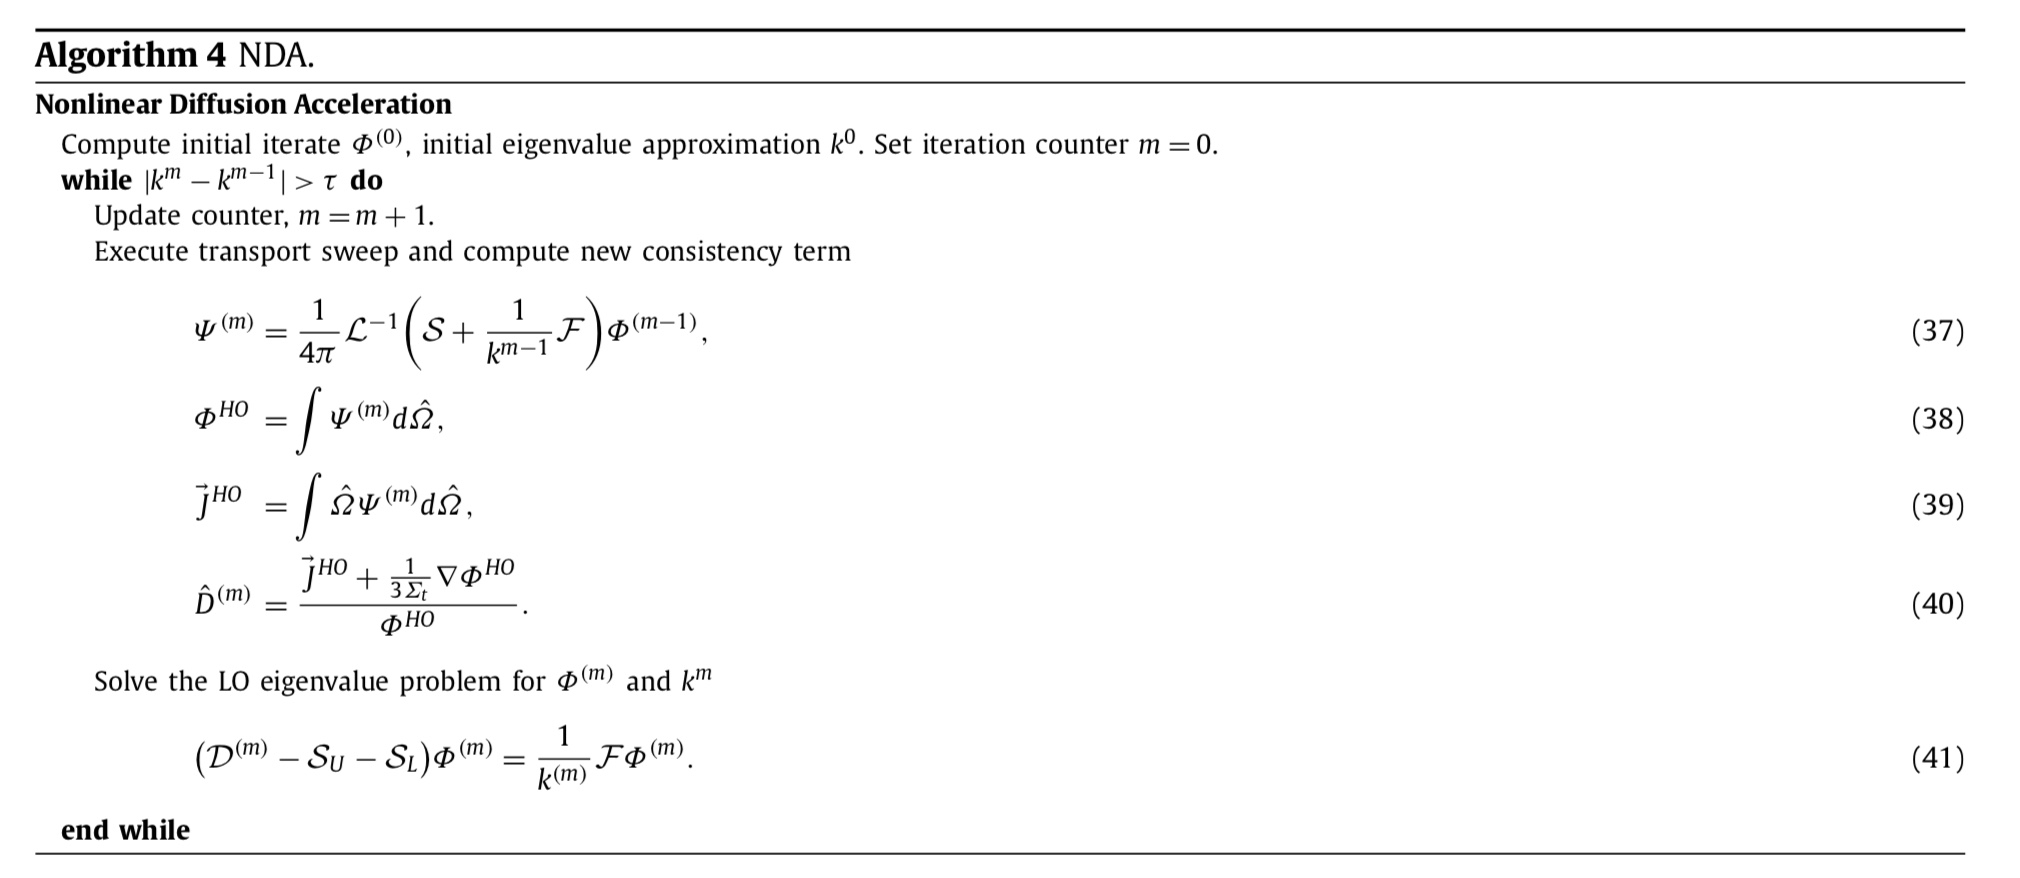
\includegraphics[width=0.95\linewidth]{algo4.jpeg}}
\end{frame}

%slide
\begin{frame}{Solving LO Eigenvalue}
Rewriting the LO problem:
\begin{equation*}
F_\Phi \left( \Phi \right) = \left( D - S_U - S_L \right) \Phi - \frac{1}{k(\Phi)} \mathscr{F} \Phi.
\end{equation*}
in which:
\begin{equation*}
k\left( \Phi \right) = \sum_{g=1}^G \int \nu \Sigma_{f,g} \phi_g dV.
\end{equation*}
Preconditioned:
\begin{equation*}
\mathscr{M} = D - S_L - \frac{1}{k^{m-1}} \mathscr{F}.
\end{equation*}
\end{frame}

%slide
\begin{frame}{Problem Set}{Dominance Ratios}
Dominance Ratio:
\begin{equation*}
 \rho = \frac{\abs{k_2}}{\abs{k_1}},
\end{equation*}
\pause
Scattering plus dominance Ratio:
\begin{equation*}
 \rho_{s+f} = \frac{\abs{k_{PI(1)}^{n+1} - k^*}}{\abs{k_{PI(1)}^n - k^*}}.
\end{equation*}
\end{frame}

%slide
\begin{frame}{Problem Set}{LRA-BWR 2g, S16, 352 x 352, $\rho = 0.97$, $\rho_{s+f} = 0.993$}
\centering
\fcolorbox{fall}{white}{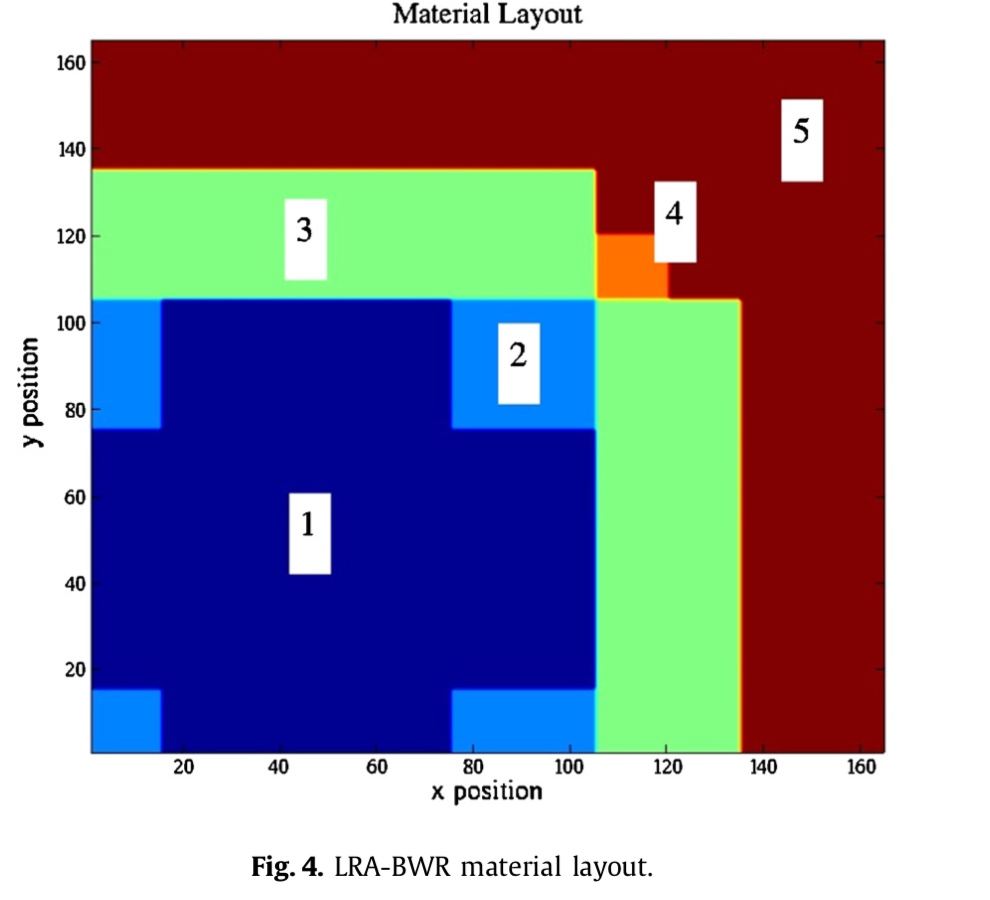
\includegraphics[width=0.45\linewidth]{fig4.jpeg}}
\end{frame}

%slide
\begin{frame}{Problem Set}{C5G7 7g, S16, 357 x 357, $\rho = 0.77$, $\rho_{s+f} = 0.989$}
\centering
\fcolorbox{fall}{white}{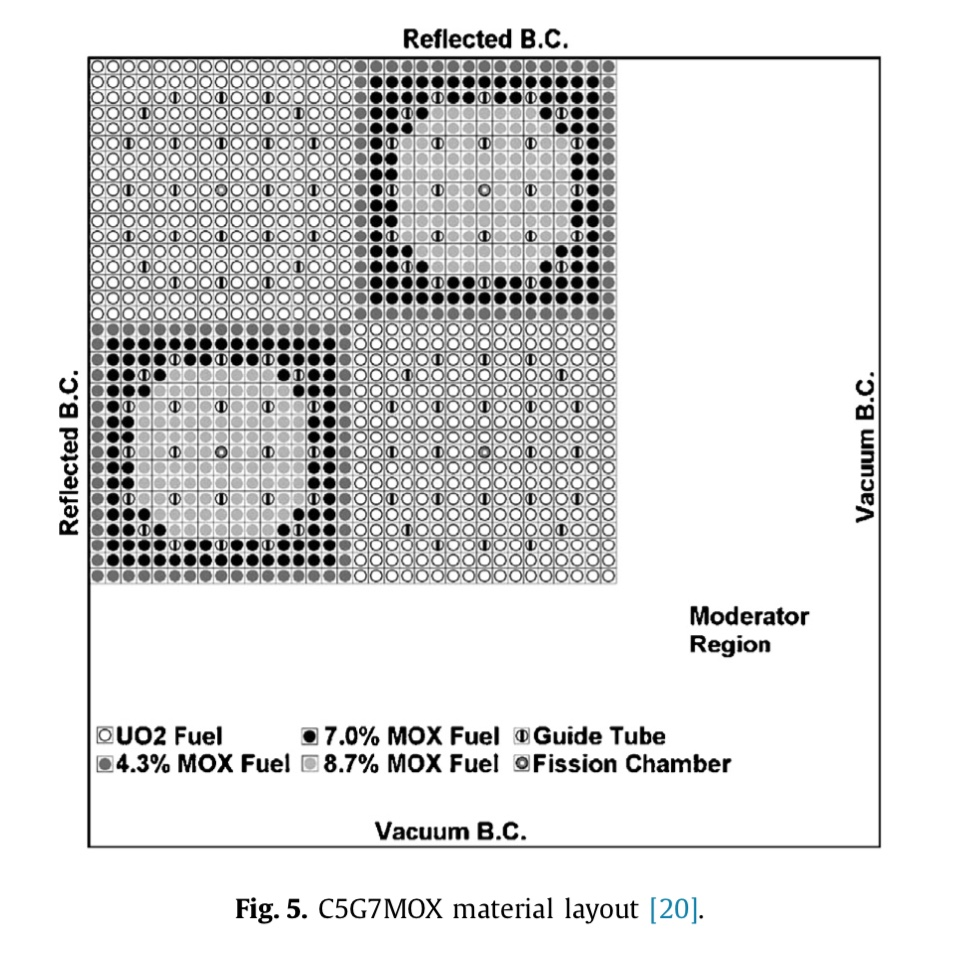
\includegraphics[width=0.45\linewidth]{fig5.jpeg}}
\end{frame}

%slide
\begin{frame}{JFNK-HO Parameter Study}
\centering
\fcolorbox{fall}{white}{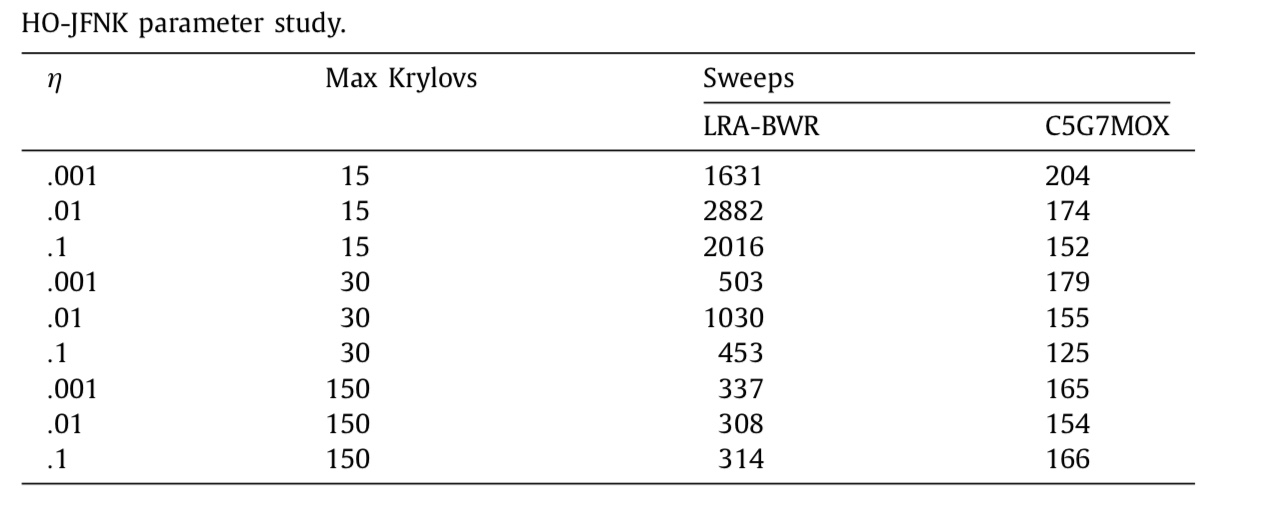
\includegraphics[width=0.85\linewidth]{table2.jpeg}}
\end{frame}

%slide
\begin{frame}{JFNK-HO vs NKA-HO Study}
\centering
\fcolorbox{fall}{white}{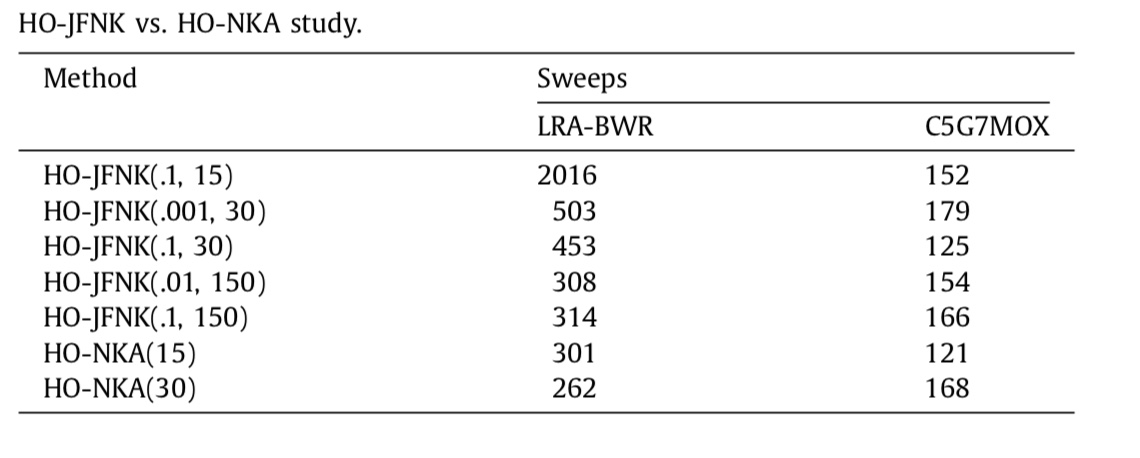
\includegraphics[width=0.85\linewidth]{table3.jpeg}}
\end{frame}

%slide
\begin{frame}{Mesh Convergence Study}{NDA-NCA}
\centering
\fcolorbox{fall}{white}{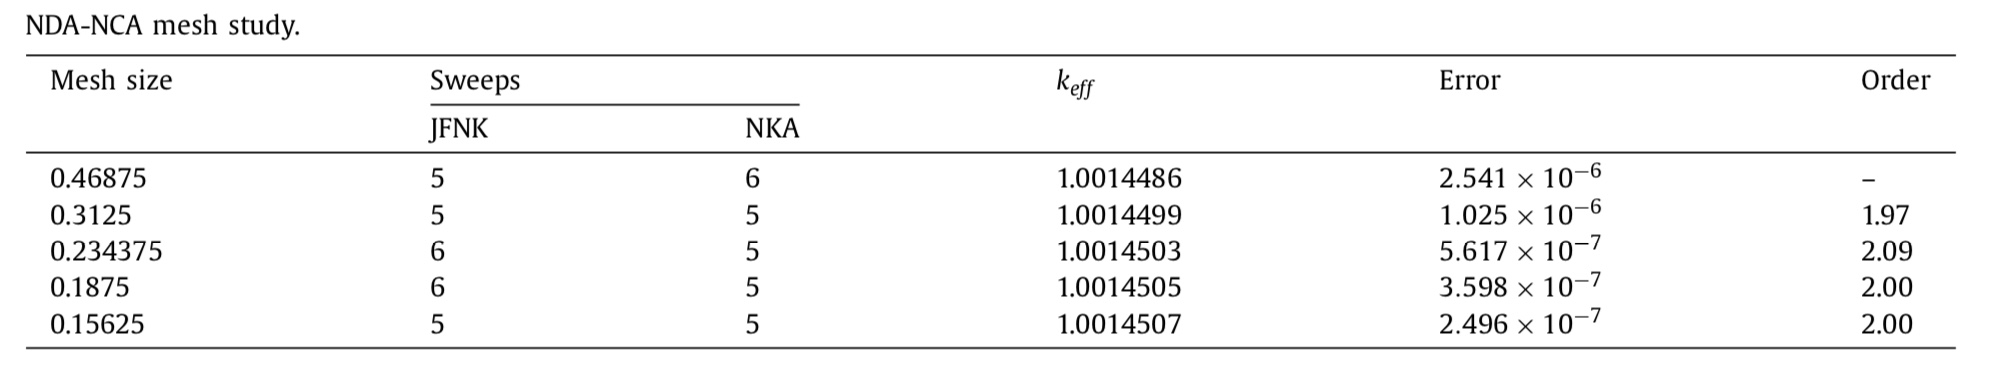
\includegraphics[width=0.99\linewidth]{table4.jpeg}}
\end{frame}

\begin{frame}{Mesh Convergence Study}{HO-NKA}
\centering
\fcolorbox{fall}{white}{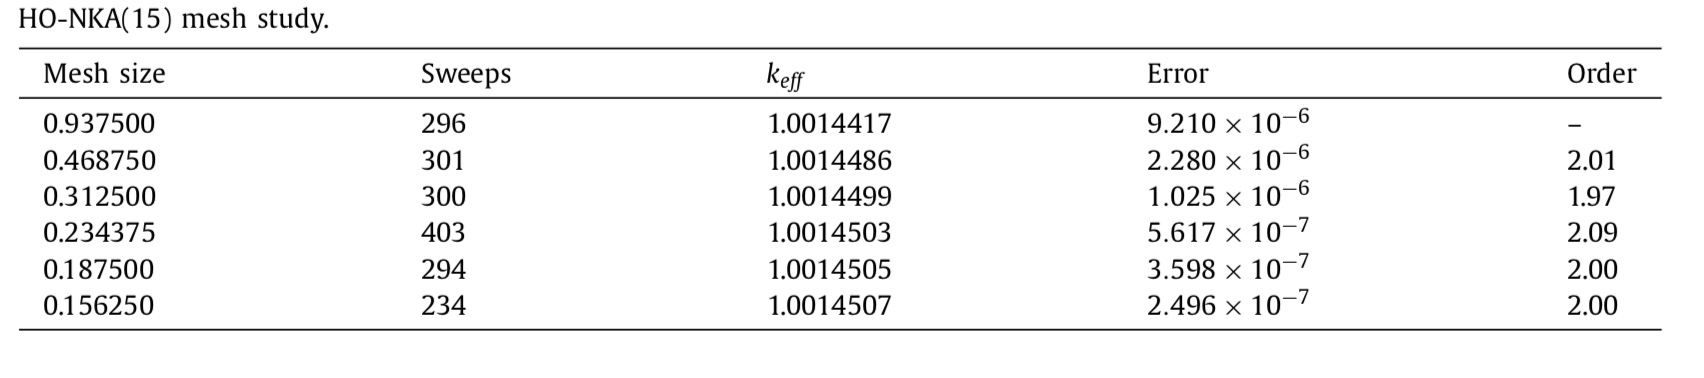
\includegraphics[width=0.99\linewidth]{table5.jpeg}}
\end{frame}

\begin{frame}{HOLO vs HO Study}{LRA-BWR}
\centering
\fcolorbox{fall}{white}{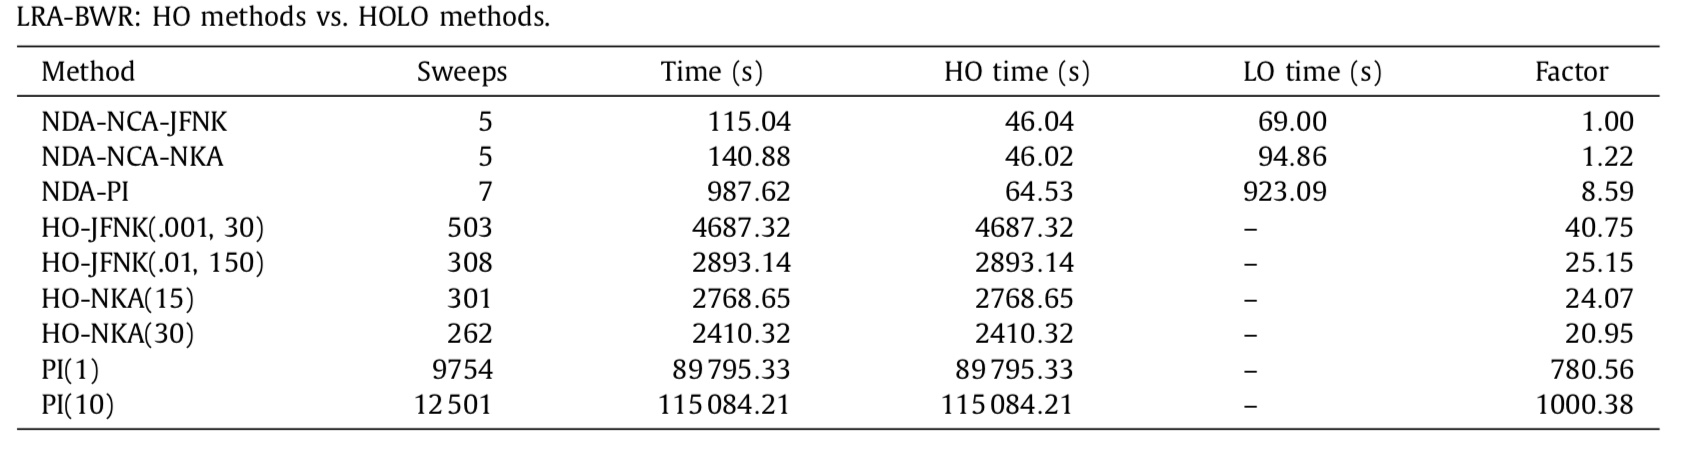
\includegraphics[width=0.99\linewidth]{table6.jpeg}}
\end{frame}

\begin{frame}{HOLO vs HO Study}{LRA-BWR: cost breakdown}
\centering
\fcolorbox{fall}{white}{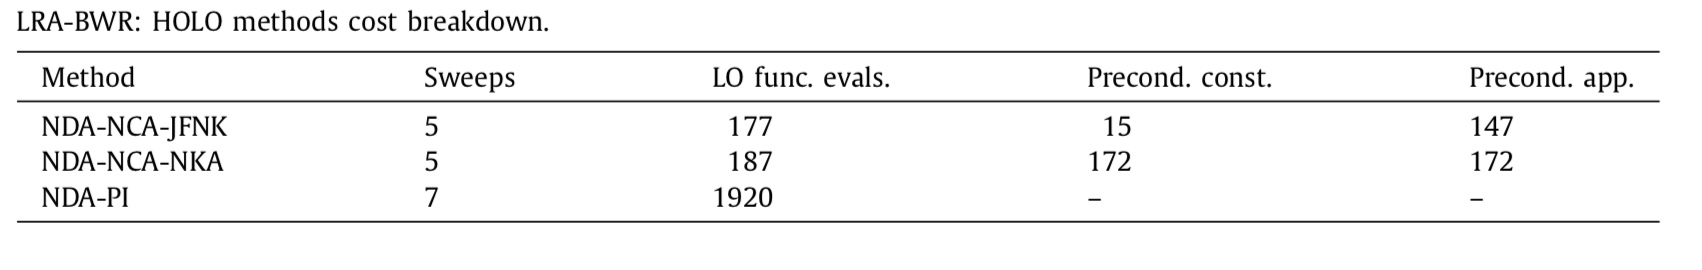
\includegraphics[width=0.99\linewidth]{table7.jpeg}}
\end{frame}

\begin{frame}{HOLO vs HO Study}{C5G7}
\centering
\fcolorbox{fall}{white}{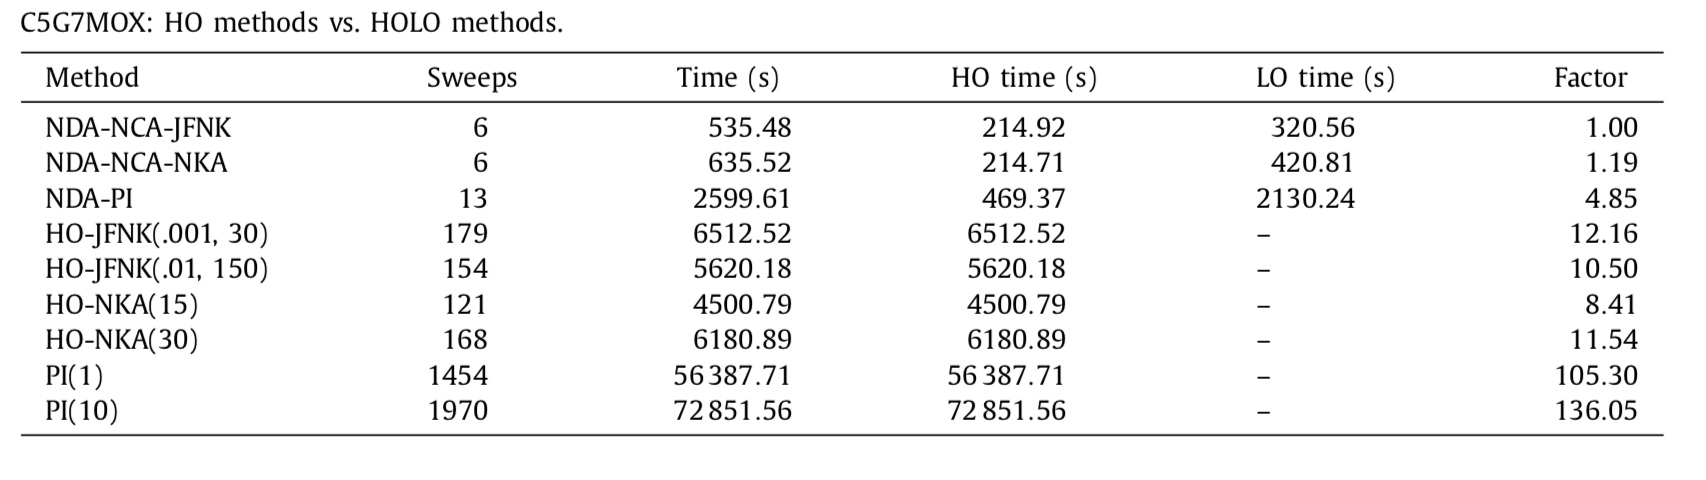
\includegraphics[width=0.99\linewidth]{table8.jpeg}}
\end{frame}

\begin{frame}{HOLO vs HO Study}{C5G7: cost breakdown}
\centering
\fcolorbox{fall}{white}{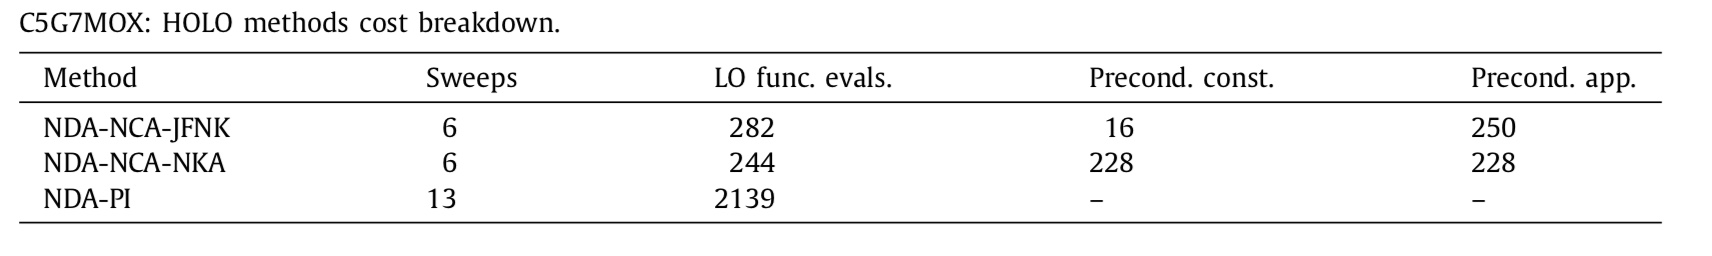
\includegraphics[width=0.99\linewidth]{table9.jpeg}}
\end{frame}

\begin{frame}{Conclusion}
\begin{itemize}
 \item NKA is \emph{generally} more efficient at solving the nonlinear HO problem.
 \item By moving a large portion of the problem to the LO computational space, overall work is reduced considerably. 
 \item While JFNK and NKA applied to the HO problem can accelerate the solution when comparted to standard power iteration, they are significantly  more expensive than
       NDA-NCA.
 \item NDA-NCA performance is less sensitive to mesh size and choice of parameters.
 \item NDA-NCA can also be preconditioned to further accelerate the solution.
 \item For both problems, BWR-LRA and C5G7, NDA-NCA is the most efficient by a factor of 10-40.
\end{itemize}
\end{frame}

%slide
\begin{frame}
\centering
\Huge
Thanks! \\
Questions?
\end{frame}


\end{document}
